\documentclass[11pt]{article}
\usepackage{graphicx}
\usepackage{hyperref}
\usepackage{longtable}
\usepackage[margin=.7in]{geometry}

\begin{document}

\title{CSE564 Visualization}
\author{Yinlong Su, \#110461173}
\maketitle

\section*{Country Eigens Report}

\setcounter{section}{-1}
\section{Version History}

First built on April 25, 2016.

\section{Country Eigens}

In order to obtain the characteristics of the foods of different countries, we need to calculate and create country eigenvectors. We select 10 attributes of the food ingredients and 135 countries to perform the task.

\section{Selected Attributes Statistics}

The selected attributes must be representative. That is to say, the attributes need to be good indicators of nutrition and health. Besides, the attributes must be relatively complete in our database. Otherwise we do not have enough data to support our calculation.
\par
The 10 attributes are:
\par
\begin{enumerate}
\item Addtivies
\item Energy
\item Fat
\item Carbohydrates
\item Sugars
\item Fiber
\item Proteins
\item Salt
\item Sodium
\item Alcohol
\end{enumerate}

Table \ref{tab:attributesTable} shows the statistics on the selected attributes. \textbf{Count} means valid data number of this attribute. \textbf{Std} means the standard deviation.
\par

\begin{center}
\begin{longtable}{|l|r|r|r|r|r|r|r|r|r|}
\caption[Selected Attributes Table]{Selected Attributes Table} \label{tab:attributesTable} \\
\hline
\multicolumn{1}{|c|}{\textbf{Column}} & \multicolumn{1}{|c|}{\textbf{Invalid}} & \multicolumn{1}{c|}{\textbf{Count}} & \multicolumn{1}{c|}{\textbf{Sum}} & \multicolumn{1}{c|}{\textbf{Min}} & \multicolumn{1}{c|}{\textbf{Max}} & \multicolumn{1}{c|}{\textbf{Avg}} & \multicolumn{1}{c|}{\textbf{Med}} & \multicolumn{1}{c|}{\textbf{Std}} \\
\hline
\endfirsthead

\multicolumn{9}{c}%
{{\bfseries \tablename\ \thetable{} -- continued from previous page}} \\
\hline
\multicolumn{1}{|c|}{\textbf{Column}} & \multicolumn{1}{|c|}{\textbf{Invalid}} & \multicolumn{1}{c|}{\textbf{Count}} & \multicolumn{1}{c|}{\textbf{Sum}} & \multicolumn{1}{c|}{\textbf{Min}} & \multicolumn{1}{c|}{\textbf{Max}} & \multicolumn{1}{c|}{\textbf{Avg}} & \multicolumn{1}{c|}{\textbf{Med}} & \multicolumn{1}{c|}{\textbf{Std}} \\
\hline
\endhead

\hline \multicolumn{9}{|r|}{{Continued on next page}} \\
\hline
\endfoot

\hline
\hline
\endlastfoot

% additives\_n & 43664 & 21822 & 76235.0 & 0.0 & 26.0 & 1.74594631733 & 1.0 & 6.25382549294 \\
% energy\_100g & 36374 & 29112 & 39116285.887 & 0.0 & 4134.0 & 1075.39137535 & 977.0 & 618417.569296 \\
% fat\_100g & 36362 & 29124 & 473736.915633 & 0.0 & 101.0 & 13.0283514557 & 5.8 & 296.576888794 \\
% carbohydrates\_100g & 36065 & 29421 & 1007295.6279 & 0.0 & 139.0 & 27.9300049328 & 14.1 & 766.599243737 \\
% sugars\_100g & 32637 & 32849 & 420724.2617 & 0.0 & 105.0 & 12.8910212857 & 4.1 & 336.582967774 \\
% fiber\_100g & 22537 & 42949 & 63445.97536 & 0.0 & 94.8 & 2.81519170076 & 1.8 & 16.4028474751 \\
% proteins\_100g & 35930 & 29556 & 266084.3289 & 0.0 & 86.0 & 7.40563119677 & 5.8 & 55.3868430378 \\
% salt\_100g & 32908 & 32578 & 36832.1327245 & 0.0 & 254.0 & 1.11924555502 & 0.508 & 19.947795762 \\
% sodium\_100g & 32898 & 32588 & 14460.545192 & 0.0 & 100.0 & 0.439556969784 & 0.2 & 3.04610859628 \\
% alcohol\_100g & 2419 & 63067 & 20564.799 & 0.0 & 97.9 & 8.50136378669 & 5.2 & 123.020155849 \\

additives\_n & 43664 & 21822 & 76235.0 & 0.0 & 26.0 & 1.75 & 1.0 & 6.25 \\
energy\_100g & 36374 & 29112 & 39116285.89 & 0.0 & 4134.0 & 1075.39 & 977.0 & 618417.57 \\
fat\_100g & 36362 & 29124 & 473736.92 & 0.0 & 101.0 & 13.03 & 5.8 & 296.58 \\
carbohydrates\_100g & 36065 & 29421 & 1007295.63 & 0.0 & 139.0 & 27.93 & 14.1 & 766.60 \\
sugars\_100g & 32637 & 32849 & 420724.26 & 0.0 & 105.0 & 12.89 & 4.1 & 336.58 \\
fiber\_100g & 22537 & 42949 & 63445.98 & 0.0 & 94.8 & 2.82 & 1.8 & 16.40 \\
proteins\_100g & 35930 & 29556 & 266084.33 & 0.0 & 86.0 & 7.41 & 5.8 & 55.39 \\
salt\_100g & 32908 & 32578 & 36832.13 & 0.0 & 254.0 & 1.12 & 0.508 & 19.95 \\
sodium\_100g & 32898 & 32588 & 14460.55 & 0.0 & 100.0 & 0.44 & 0.2 & 3.05 \\
alcohol\_100g & 2419 & 63067 & 20564.80 & 0.0 & 97.9 & 8.50 & 5.2 & 123.02 \\

\hline

\end{longtable}
\end{center}

Figure \ref{fig:attributesValidityFigure} shows the valid percentage of the selected attributes. The sub-bar shows the distributions of the average within each attribute.

\begin{figure}[!htp]
\centering
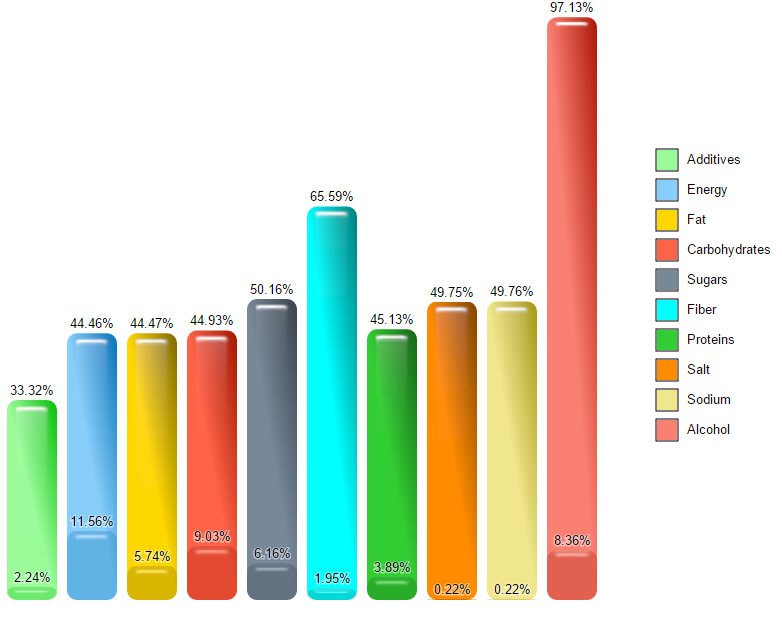
\includegraphics[width=\textwidth]{../vis/selected.attributes.validity.png}
\caption{Validities of Attributes}
\label{fig:attributesValidityFigure}
\end{figure}

\section{Country Eigenvectors}
Table \ref{tab:eigenvectorsTable} shows the eigenvectors of 10 attributes and 135 countries.

\begin{center}
\begin{longtable}{|p{70pt}|r|r|r|r|r|r|r|r|r|r|}
\caption[Eigenvectors Table]{Eigenvectors Table} \label{tab:eigenvectorsTable} \\
\hline
\multicolumn{1}{|c|}{\textbf{Country Name}} & \multicolumn{1}{c|}{\textbf{Adds}} & \multicolumn{1}{c|} {\textbf{E}} & \multicolumn{1}{c|}{\textbf{Fat}} & \multicolumn{1}{c|}{\textbf{Carbs}} & \multicolumn{1}{c|}{\textbf{Sugars}} & \multicolumn{1}{c|}{\textbf{Fiber}} & \multicolumn{1}{c|}{\textbf{Prot}} & \multicolumn{1}{c|}{\textbf{Salt}} & \multicolumn{1}{c|}{\textbf{Sodium}} & \multicolumn{1}{c|}{\textbf{Alcohol}} \\
\hline
\endfirsthead

\multicolumn{11}{c}%
{{\bfseries \tablename\ \thetable{} -- continued from previous page}} \\
\hline
\multicolumn{1}{|c|}{\textbf{Country Name}} & \multicolumn{1}{c|}{\textbf{Adds}} & \multicolumn{1}{c|} {\textbf{E}} & \multicolumn{1}{c|}{\textbf{Fat}} & \multicolumn{1}{c|}{\textbf{Carbs}} & \multicolumn{1}{c|}{\textbf{Sugars}} & \multicolumn{1}{c|}{\textbf{Fiber}} & \multicolumn{1}{c|}{\textbf{Prots}} & \multicolumn{1}{c|}{\textbf{Salt}} & \multicolumn{1}{c|}{\textbf{Sodium}} & \multicolumn{1}{c|}{\textbf{Alcohol}} \\
\hline
\endhead

\hline \multicolumn{11}{|r|}{{Continued on next page}} \\
\hline
\endfoot

\hline
\hline
\endlastfoot

Romania& 0.07& 0.37& 0.14& 0.41& 0.21& 0.03& 0.08& 0.0& 0.0& 0.02\\
Malta& 0.05& 0.2& 0.09& 0.19& 0.02& 0.02& 0.05& 0.0& 0.0& 0.13\\
Kuwait& 0.12& 0.02& 0.0& 0.05& 0.06& nan& 0.0& 0.01& 0.01& nan\\
Sweden& 0.01& 0.28& 0.1& 0.26& 0.19& 0.08& 0.09& 0.0& 0.0& 0.05\\
United Kingdom& 0.05& 0.27& 0.14& 0.2& 0.16& 0.02& 0.08& 0.0& 0.0& 0.13\\
Iran& 0.0& nan& nan& nan& nan& nan& nan& nan& nan& nan\\
Norway& 0.06& 0.34& 0.13& 0.35& 0.22& 0.02& 0.05& 0.0& 0.0& 0.05\\
Hungary& 0.02& 0.38& 0.24& 0.23& 0.03& 0.04& 0.11& 0.0& 0.0& 0.07\\
Canada& 0.07& 0.25& 0.11& 0.22& 0.17& 0.03& 0.06& 0.0& 0.0& 0.02\\
France& 0.07& 0.26& 0.13& 0.2& 0.12& 0.03& 0.09& 0.0& 0.0& 0.09\\
Polska& 0.0& 0.05& 0.0& 0.09& 0.11& nan& 0.0& 0.0& 0.0& nan\\
Japan& 0.03& 0.25& 0.08& 0.31& 0.46& 0.04& 0.05& 0.01& 0.01& nan\\
Greece& 0.04& 0.28& 0.12& 0.22& 0.12& 0.03& 0.09& 0.0& 0.0& 0.07\\
Estonia& nan& nan& nan& nan& nan& nan& nan& nan& nan& nan\\
Senegal& 0.07& 0.37& 0.18& 0.32& 0.21& 0.03& 0.09& 0.0& 0.0& nan\\
Israel& 0.04& 0.25& 0.14& 0.19& 0.01& 0.0& 0.03& 0.01& 0.01& 0.05\\
Argentina& 0.07& 0.22& 0.07& 0.25& 0.08& 0.01& 0.03& 0.0& 0.0& 0.08\\
Morocco& 0.13& 0.31& 0.14& 0.29& 0.24& 0.02& 0.06& 0.0& 0.0& 0.06\\
Kazakhstan& nan& nan& nan& nan& nan& nan& nan& nan& nan& nan\\
Thailanda& 0.0& 0.25& 0.2& 0.09& 0.1& 0.06& 0.05& 0.03& 0.03& nan\\
Russia& 0.0& 0.38& 0.25& 0.25& 0.03& 0.01& 0.11& 0.0& 0.0& 0.12\\
Belize& nan& 0.05& 0.02& 0.03& nan& nan& 0.04& nan& nan& nan\\
South Korea& 0.08& 0.37& 0.13& 0.39& 0.05& 0.0& 0.09& 0.01& 0.01& 0.0\\
Mayotte& 0.0& nan& nan& nan& nan& nan& nan& nan& nan& nan\\
Cambodia& 0.01& 0.21& 0.12& 0.17& 0.11& 0.01& 0.1& 0.0& 0.0& 0.05\\
Spain& 0.04& 0.24& 0.13& 0.18& 0.1& 0.04& 0.07& 0.0& 0.0& 0.05\\
Albania& 0.01& 0.26& 0.06& 0.26& 0.09& 0.02& 0.12& 0.0& 0.0& 0.07\\
Hawaii& nan& nan& nan& nan& nan& nan& nan& nan& nan& nan\\
Dominican Republic& nan& nan& nan& nan& nan& nan& nan& nan& nan& nan\\
Egypt& 0.21& 0.28& 0.12& 0.26& 0.31& 0.01& 0.05& 0.0& 0.0& nan\\
South Africa& 0.07& 0.36& 0.28& 0.14& 0.07& 0.03& 0.08& 0.0& 0.0& 0.0\\
Bangladesh& nan& nan& nan& nan& nan& nan& nan& nan& nan& nan\\
Iraq& 0.06& 0.05& 0.0& 0.08& 0.11& nan& 0.0& 0.0& 0.0& nan\\
Kenya& 0.06& 0.1& 0.03& 0.09& 0.11& nan& 0.05& nan& nan& nan\\
An& 0.03& 0.44& 0.17& 0.46& 0.34& 0.09& 0.06& 0.0& 0.0& 0.13\\
Panama& nan& nan& nan& nan& nan& nan& nan& nan& nan& nan\\
Yemen& nan& nan& nan& nan& nan& nan& nan& nan& nan& nan\\
Switzerland& 0.07& 0.27& 0.13& 0.22& 0.13& 0.03& 0.08& 0.0& 0.0& 0.02\\
Tunisia& 0.09& 0.38& 0.24& 0.32& 0.28& 0.02& 0.07& 0.0& 0.0& 0.0\\
French Polynesia& 0.08& 0.34& 0.13& 0.29& 0.26& 0.08& 0.09& 0.0& 0.0& nan\\
Colombia& 0.02& 0.05& 0.03& 0.05& 0.07& 0.02& 0.04& 0.0& 0.0& nan\\
Syria& nan& nan& nan& nan& nan& nan& nan& nan& nan& nan\\
Luxembourg& 0.08& 0.26& 0.15& 0.17& 0.14& 0.01& 0.08& 0.0& 0.0& 0.06\\
New Zealand& 0.1& 0.32& 0.13& 0.28& 0.2& 0.05& 0.09& 0.0& 0.0& 0.06\\
Hong Kong& 0.05& 0.18& 0.14& 0.17& 0.08& 0.02& 0.03& 0.0& 0.0& 0.01\\
Mongolia& nan& nan& nan& nan& nan& nan& nan& nan& nan& nan\\
China& 0.05& 0.37& 0.13& 0.32& 0.01& 0.11& 0.1& 0.01& 0.01& 0.06\\
Turkey& 0.01& 0.27& 0.19& 0.31& 0.2& 0.02& 0.09& 0.0& 0.0& nan\\
Philippines& 0.03& 0.29& 0.05& 0.44& 0.46& 0.08& 0.09& 0.0& 0.0& nan\\
Nederland& 0.0& 0.67& 0.57& 0.08& 0.06& 0.07& 0.24& 0.0& 0.0& nan\\
Lebanon& 0.02& 0.29& 0.15& 0.03& 0.01& 0.04& 0.11& 0.0& 0.0& nan\\
French Guiana& 0.07& 0.22& 0.09& 0.2& 0.11& 0.03& 0.09& 0.0& 0.0& 0.03\\
Belarus& 0.0& nan& nan& nan& nan& nan& nan& nan& nan& nan\\
Italy& 0.04& 0.3& 0.12& 0.28& 0.14& 0.03& 0.09& 0.0& 0.0& 0.12\\
Mauritius& 0.08& 0.39& nan& nan& nan& nan& nan& nan& nan& 0.05\\
Croatia& nan& nan& nan& nan& nan& nan& nan& nan& nan& nan\\
Qatar& 0.17& 0.2& 0.14& 0.15& 0.51& 0.01& 0.05& 0.0& 0.0& nan\\
Irlande& 0.0& 0.39& 0.06& 0.54& 0.69& 0.03& 0.07& 0.0& 0.0& 0.0\\
Chile& 0.13& 0.25& 0.07& 0.14& 0.0& 0.0& 0.36& 0.0& 0.0& 0.0\\
Sri Lanka& 0.0& nan& nan& nan& nan& nan& nan& nan& nan& nan\\
Georgia& nan& nan& nan& nan& nan& nan& nan& nan& nan& nan\\
Republic of the Congo& nan& nan& nan& nan& nan& nan& nan& nan& nan& nan\\
Armenia& nan& nan& nan& nan& nan& nan& nan& nan& nan& 0.41\\
Martinique& 0.06& 0.12& 0.08& 0.14& 0.15& 0.03& 0.04& 0.0& 0.0& 0.03\\
Slovakia& nan& 0.05& 0.0& 0.08& 0.11& nan& 0.0& 0.0& 0.0& nan\\
Malaysia& 0.04& nan& nan& nan& nan& nan& nan& nan& nan& nan\\
Cyprus& 0.0& nan& nan& nan& nan& nan& nan& nan& nan& nan\\
Czech Republic& 0.05& 0.18& 0.08& 0.15& 0.18& 0.02& 0.04& 0.0& 0.0& 0.03\\
Lithuania& 0.04& 0.35& 0.11& 0.37& 0.29& 0.02& 0.09& 0.0& 0.0& nan\\
Burundi& nan& nan& nan& nan& nan& nan& nan& nan& nan& nan\\
Guatemala& nan& nan& nan& nan& nan& nan& nan& nan& nan& nan\\
Mexico& 0.07& 0.23& 0.1& 0.24& 0.1& 0.03& 0.04& 0.01& 0.01& nan\\
Algeria& 0.11& 0.29& 0.15& 0.22& 0.35& 0.01& 0.07& 0.0& 0.0& nan\\
Denmark& 0.06& 0.3& 0.16& 0.22& 0.17& 0.03& 0.09& 0.01& 0.01& 0.19\\
Germany& 0.03& 0.26& 0.14& 0.19& 0.12& 0.04& 0.1& 0.0& 0.0& 0.06\\
El Salvador& nan& nan& nan& nan& nan& nan& nan& nan& nan& nan\\
Cook Islands& nan& nan& nan& nan& nan& nan& nan& nan& nan& nan\\
Guadeloupe& 0.06& 0.21& 0.08& 0.18& 0.12& 0.02& 0.07& 0.0& 0.0& 0.14\\
European Union& 0.12& 0.46& 0.17& 0.47& 0.26& 0.03& 0.09& 0.0& 0.0& nan\\
United Arab Emirates& 0.07& 0.24& 0.11& 0.19& 0.32& 0.03& 0.08& 0.0& 0.0& nan\\
Guinea& nan& nan& nan& nan& nan& nan& nan& nan& nan& nan\\
Mozambique& nan& nan& nan& nan& nan& nan& nan& nan& nan& nan\\
Macau& nan& nan& nan& nan& nan& nan& nan& nan& nan& nan\\
Azerbaijan& nan& nan& nan& nan& nan& nan& nan& nan& nan& nan\\
Monaco& 0.19& 0.44& 0.15& 0.49& 0.27& 0.04& 0.06& 0.0& 0.0& nan\\
Australia& 0.02& 0.25& 0.11& 0.21& 0.15& 0.04& 0.08& 0.01& 0.01& 0.13\\
Brunei& nan& nan& nan& nan& nan& nan& nan& nan& nan& nan\\
Serbia& 0.08& 0.32& 0.11& 0.5& 0.24& 0.32& 0.1& 0.0& 0.0& nan\\
New Caledonia& 0.05& 0.24& 0.13& 0.22& 0.14& 0.06& 0.05& 0.0& 0.0& nan\\
Iceland& 0.03& nan& nan& nan& nan& nan& nan& nan& nan& nan\\
Austria& 0.02& 0.26& 0.1& 0.26& 0.13& 0.04& 0.07& 0.03& 0.03& 0.15\\
Ukraine& nan& 0.46& 0.2& 0.48& 0.19& 0.04& 0.08& 0.0& 0.0& 0.05\\
Burkina Faso& 0.06& 0.06& 0.0& 0.1& nan& nan& 0.0& nan& nan& nan\\
Portugal& 0.07& 0.28& 0.12& 0.24& 0.14& 0.03& 0.08& 0.01& 0.01& 0.13\\
Gabon& nan& nan& nan& nan& nan& nan& nan& nan& nan& nan\\
Mali& nan& nan& nan& nan& nan& nan& nan& nan& nan& nan\\
Peru& nan& nan& nan& nan& nan& nan& nan& nan& nan& nan\\
Andorra& 0.01& 0.51& 0.3& 0.36& 0.45& 0.09& 0.07& 0.0& 0.0& 0.13\\
Vanuatu& nan& nan& nan& nan& nan& nan& nan& nan& nan& nan\\
Pakistan& nan& nan& nan& nan& nan& nan& nan& nan& nan& nan\\
Ghana& nan& nan& nan& nan& nan& nan& nan& nan& nan& nan\\
Saint Pierre and Miquelon& 0.09& 0.26& 0.15& 0.22& 0.12& 0.03& 0.05& 0.0& 0.0& 0.0\\
Finland& 0.02& 0.44& 0.18& 0.44& 0.31& 0.02& 0.05& 0.0& 0.0& 0.07\\
Ireland& 0.03& 0.44& 0.39& 0.24& 0.1& 0.02& 0.07& 0.0& 0.0& 0.02\\
Latvia& nan& nan& nan& nan& nan& nan& nan& nan& nan& nan\\
Tanzania& nan& nan& nan& nan& nan& nan& nan& nan& nan& nan\\
Togo& 0.31& 0.06& nan& 0.1& nan& nan& nan& nan& nan& nan\\
Moldova& nan& 0.53& 0.33& 0.35& 0.02& 0.05& 0.08& 0.0& 0.0& nan\\
Poland& 0.09& 0.23& 0.12& 0.16& 0.15& 0.02& 0.06& 0.01& 0.01& 0.16\\
Venezuela& 0.0& 0.02& 0.0& 0.14& 0.09& nan& 0.07& nan& nan& nan\\
Aruba& nan& 0.48& 0.17& 0.5& 0.08& 0.01& 0.09& 0.01& 0.01& nan\\
Belgium& 0.07& 0.28& 0.14& 0.22& 0.14& 0.04& 0.07& 0.0& 0.0& 0.06\\
Brazil& 0.03& 0.31& 0.12& 0.32& 0.21& 0.04& 0.07& 0.01& 0.01& 0.03\\
Bahrain& nan& nan& nan& nan& nan& nan& nan& nan& nan& nan\\
Sint Maarten& nan& nan& nan& nan& nan& nan& nan& nan& nan& nan\\
Slovenia& 0.01& 0.4& 0.15& 0.39& 0.21& 0.05& 0.09& 0.0& 0.0& 0.05\\
United States& 0.08& 0.28& 0.14& 0.25& 0.16& 0.03& 0.08& 0.01& 0.01& 0.07\\
Singapore& 0.04& 0.15& 0.07& 0.14& 0.05& 0.02& 0.06& 0.01& 0.01& 0.05\\
Taiwan& 0.0& 0.06& 0.0& 0.04& 0.06& 0.0& 0.01& 0.0& 0.0& 0.0\\
Costa Rica& nan& nan& nan& nan& nan& nan& nan& nan& nan& nan\\
Cuba& 0.07& 0.28& 0.16& 0.22& 0.05& 0.03& 0.02& 0.0& 0.0& 0.41\\
Mauritania& nan& nan& nan& nan& nan& nan& nan& nan& nan& nan\\
Ecuador& nan& nan& nan& nan& nan& nan& nan& nan& nan& nan\\
Thailand& 0.03& 0.19& 0.07& 0.19& 0.08& 0.02& 0.08& 0.02& 0.02& 0.03\\
Netherlands& 0.06& 0.32& 0.13& 0.32& 0.22& 0.04& 0.08& 0.01& 0.01& 0.06\\
Vietnam& nan& nan& nan& nan& nan& nan& nan& nan& nan& nan\\
Scotland& 0.05& 0.22& 0.08& 0.19& 0.05& 0.03& 0.11& 0.0& 0.0& 0.09\\
Indonesia& 0.08& 0.33& 0.11& 0.38& 0.24& 0.03& 0.06& 0.01& 0.01& nan\\
Democratic Republic of the Congo& nan& nan& nan& nan& nan& nan& nan& nan& nan& nan\\
Niger& nan& nan& nan& nan& nan& nan& nan& nan& nan& nan\\
Saudi Arabia& 0.15& 0.2& 0.09& 0.19& 0.51& nan& 0.05& 0.0& 0.0& nan\\
Maldives& nan& nan& nan& nan& nan& nan& nan& nan& nan& nan\\
Bulgaria& 0.05& 0.33& 0.17& 0.22& 0.32& 0.03& 0.05& 0.0& 0.0& nan\\
Jordan& nan& nan& nan& nan& nan& nan& nan& nan& nan& nan\\
India& 0.08& 0.12& 0.13& 0.29& 0.16& 0.03& 0.1& 0.0& 0.0& 0.0\\

\hline

\end{longtable}
\end{center}

\par
Among those eigenvectors, we should remove some countries that have no supporting data. Perhaps remove or change some attributes too. Further work still need to be done.

\section{Visualization on eigenvectors}
We removed the countries which have at least 5 nan values (half of 10 attributes). For those nan values remained, we substitution them with $0$. Therefore 50 countries were removed and 50 nan values were filled with $0$. Then we perform PCA, MDS - Euclidean, MDS - Cosine, MDS - Correlation and ISOMAP on the new matrix to visualize the eigenvectors. Figure \ref{fig:pcaEigenvectorsFigure}, \ref{fig:mdsEuclideanEigenvectorsFigure}, \ref{fig:mdsCosineEigenvectorsFigure}, \ref{fig:mdsCorrelationEigenvectorsFigure} and \ref{fig:isomapEigenvectorsFigure} show the minimum spanning tree of the results.

\begin{figure}[!htp]
\centering
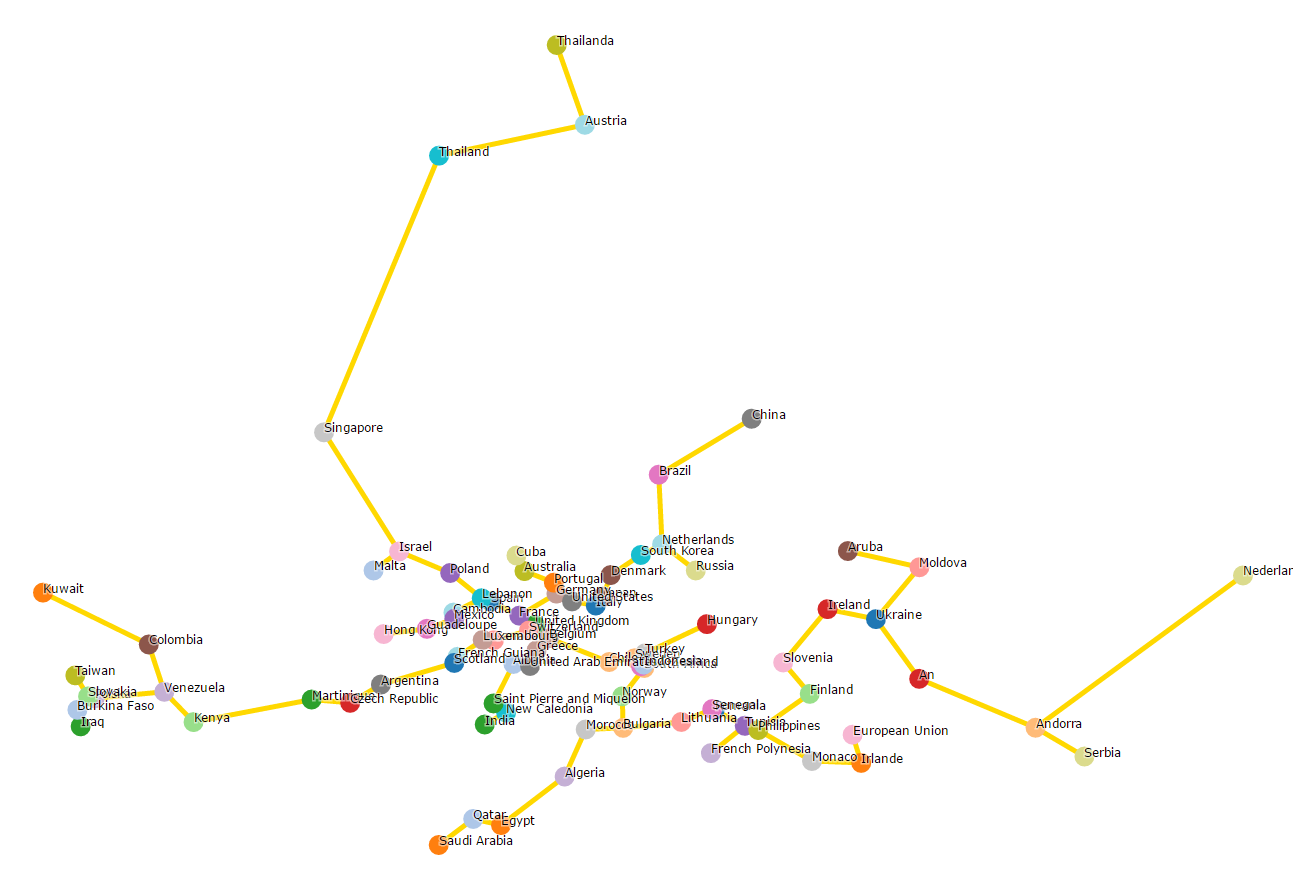
\includegraphics[width=\textwidth]{../vis/country.eigens.vis.pca.png}
\caption{PCA on eigenvectors}
\label{fig:pcaEigenvectorsFigure}
\end{figure}

\begin{figure}[!htp]
\centering
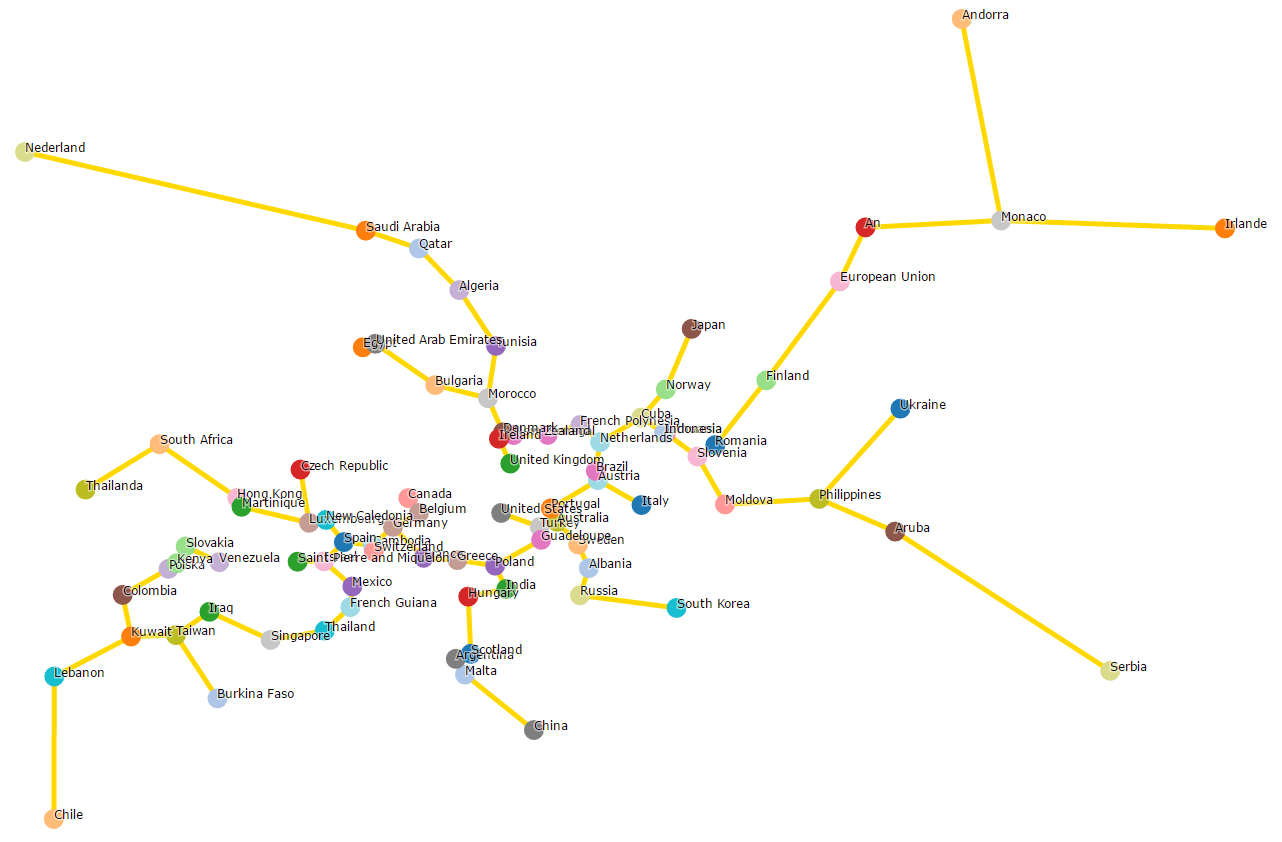
\includegraphics[width=\textwidth]{../vis/country.eigens.vis.mds.euclidean.png}
\caption{MDS - Euclidean on eigenvectors}
\label{fig:mdsEuclideanEigenvectorsFigure}
\end{figure}

\begin{figure}[!htp]
\centering
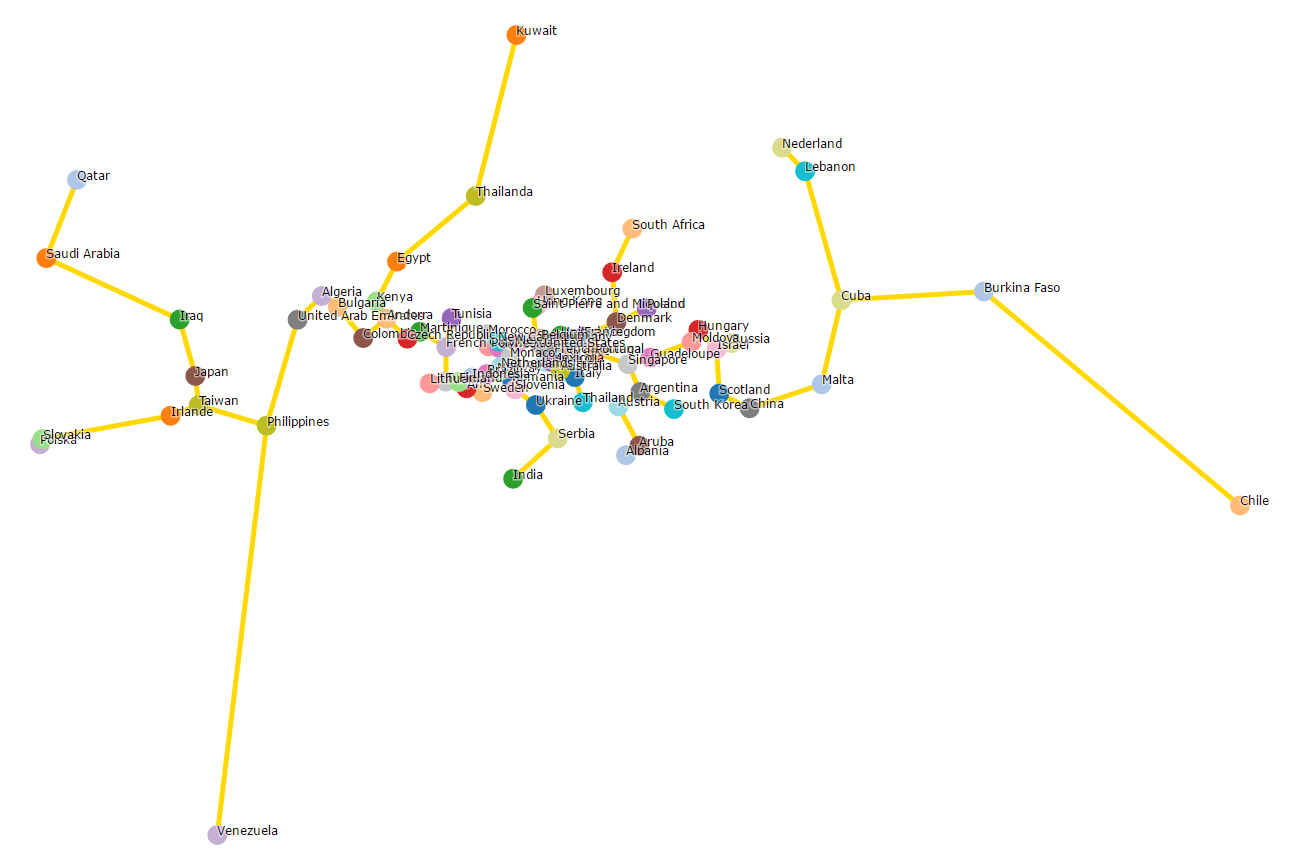
\includegraphics[width=\textwidth]{../vis/country.eigens.vis.mds.cosine.png}
\caption{MDS - Cosine on eigenvectors}
\label{fig:mdsCosineEigenvectorsFigure}
\end{figure}

\begin{figure}[!htp]
\centering
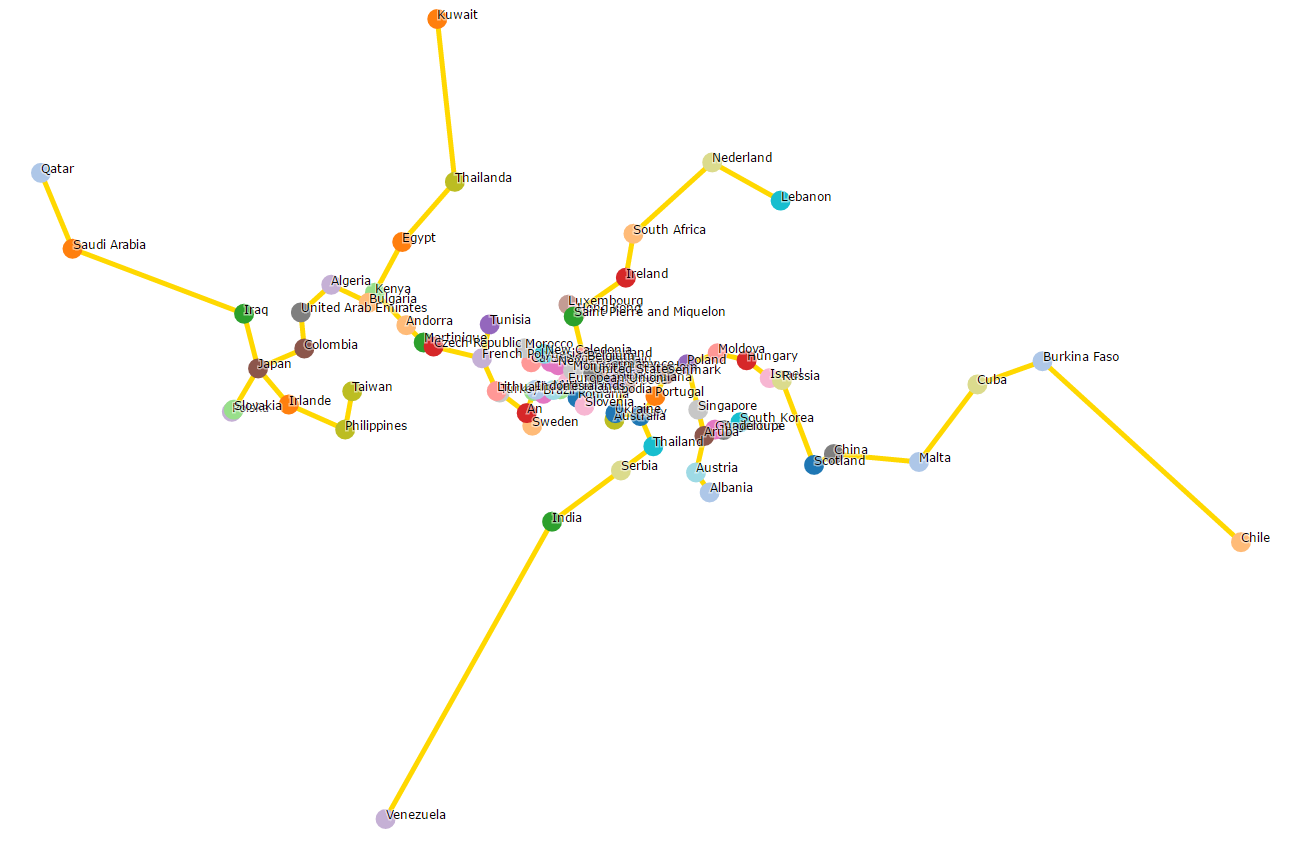
\includegraphics[width=\textwidth]{../vis/country.eigens.vis.mds.correlation.png}
\caption{MDS - Correlation on eigenvectors}
\label{fig:mdsCorrelationEigenvectorsFigure}
\end{figure}

\begin{figure}[!htp]
\centering
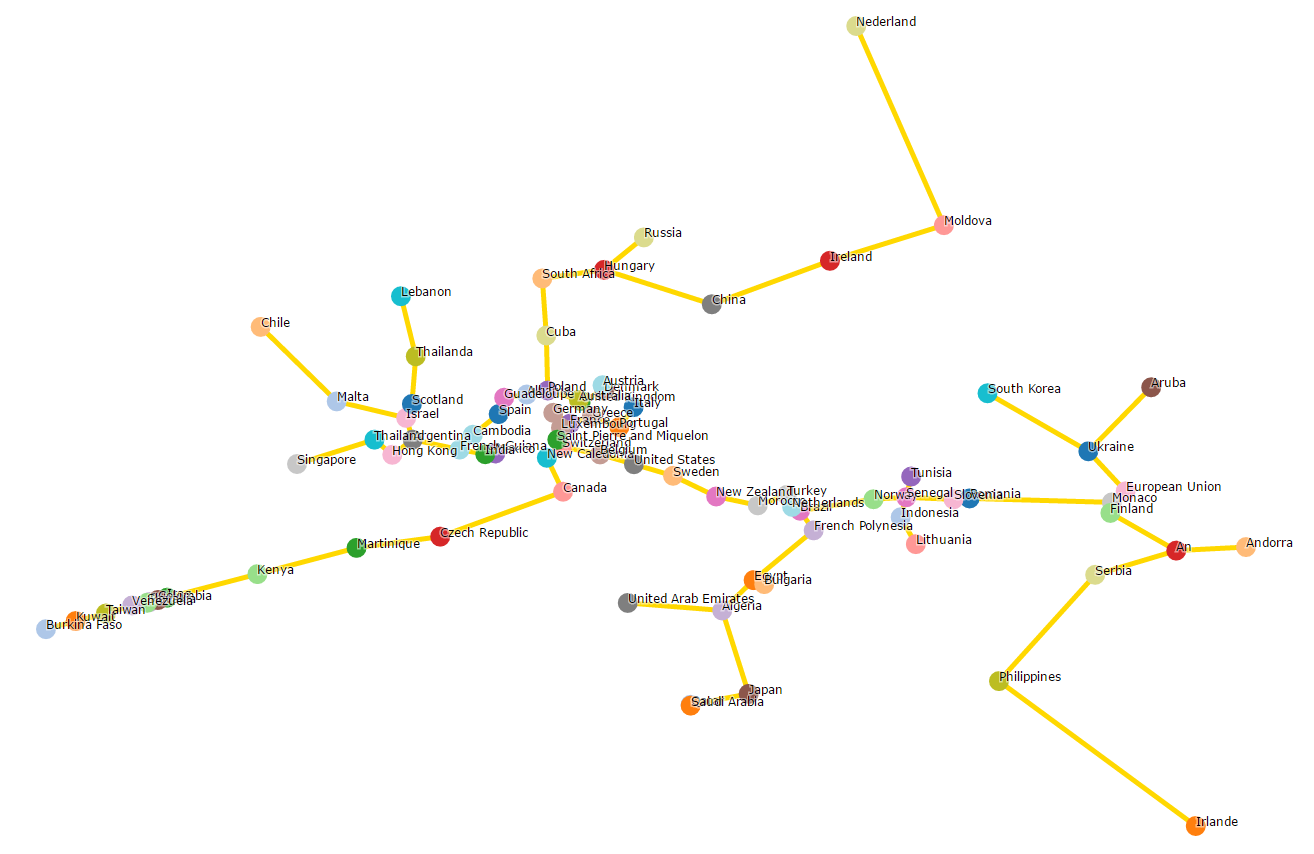
\includegraphics[width=\textwidth]{../vis/country.eigens.vis.isomap.png}
\caption{ISOMAP on eigenvectors}
\label{fig:isomapEigenvectorsFigure}
\end{figure}

\section{Contact Information}
If there is any problem please contact me.
\par
Name: Yinlong Su
\par
SBU ID: 110461173
\par
Email: yinlsu@cs.stonybrook.edu

\end{document}
